\documentclass{beamer} 


%======================================================================
% Packages / Options
%======================================================================

\usepackage[utf8]{inputenc}
\usepackage[T1]{fontenc}
\usepackage{listings}
\usepackage{fancyvrb}
\lstset{language=caml,basicstyle=\ttfamily}

% Beamer-specific settings
\mode<presentation>
{
  \usetheme{Darmstadt}
  \useoutertheme{infolines}
}

\AtBeginSection[]
{
  \begin{frame}<beamer>
    \frametitle{Plan}
    \tableofcontents[sectionstyle=show/shaded,subsectionstyle=hide]
  \end{frame}
}

\AtBeginSubsection[]
{
  \begin{frame}<beamer>
    \frametitle{Plan}
    \tableofcontents[sectionstyle=show/hide,subsectionstyle=show/shaded/hide]
  \end{frame}
}

\setbeamertemplate{footline}
{%
\insertpagenumber
\insertshorttitle[width={3cm},center]
\insertshortinstitute[width={3cm},center]
\insertshortdate[width={3cm},center]
}


%======================================================================
% Titlepage
%======================================================================

\title[Analyse Syntaxique]{Analyse Syntaxique}

\author{Mohammed Akram RHAFRANE - Mehdi BOUTCHICHE - Nathanael BERTRAND - Ismail SENHAJI}
\institute{Université de Toulouse III/IRIT}
\date{Année 2012/2013} 

\begin{document}

\begin{frame}
  \titlepage
\end{frame}


%======================================================================
\section{Objectifs du TER}\label{sec:Objectifs}

\begin{frame}\frametitle{Objectif du TER}

	\begin{itemize}
	\item Initiation à la recherche bibliographique\newline

	\item Rédaction :\newline
				\subitem \textit{Rapport sur le sujet (40 pages)}\newline
				\subitem \textit{Rapport du TER (10 pages)}\newline
				\subitem \textit{Présentation du TER}\newline			

	\item Tous les livrables sont rédigés en Latex
	\end{itemize}

\end{frame}

% Section 1---------------------------------------------------
\section{Fondamentaux}

\subsection{Contexte}

\begin{frame}\frametitle{Contexte}

	\begin{figure}[h]
		\centering
			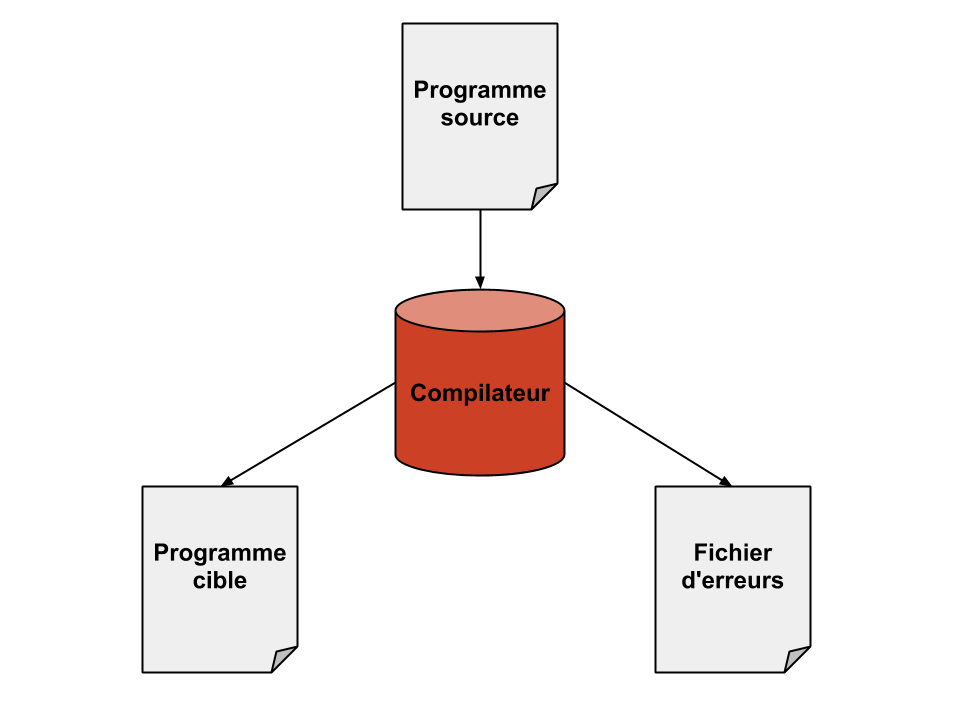
\includegraphics[width=0.65\textwidth]{compilateur.png}
		\caption{Compilateur}
		\label{fig:compilateur}
	\end{figure}\FloatBarrier

\end{frame}

\begin{frame}\frametitle{Contexte}

	\begin{figure}[h]
		\centering
			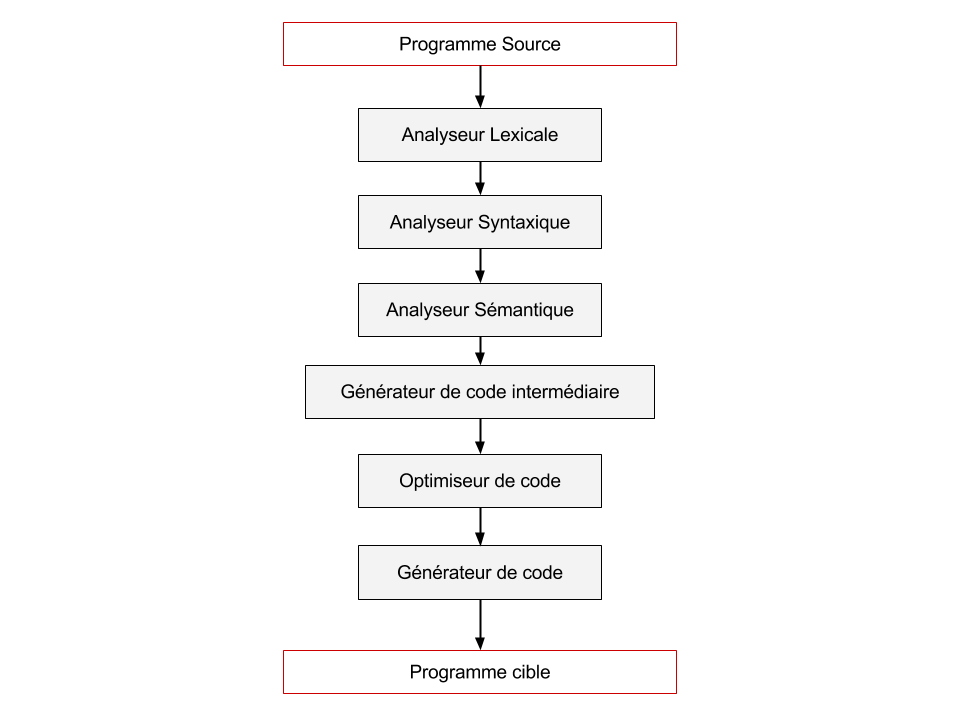
\includegraphics[width=0.65\textwidth]{compilation.png}
		\caption{Processus de compilation}
		\label{fig:compilation}
	\end{figure}\FloatBarrier

\end{frame}

\subsection{Analyse Lexicale}

\begin{frame}\frametitle{Analyse Lexicale}\framesubtitle{Principe}

	\begin{figure}[h]
		\centering
			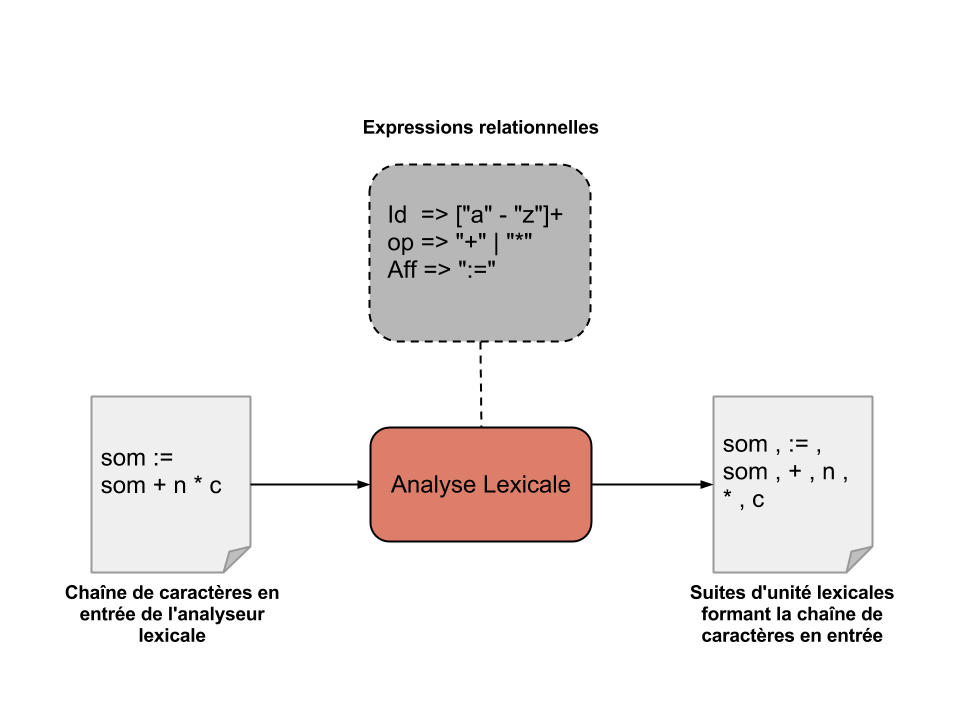
\includegraphics[width=0.65\textwidth]{AnalyseLexicale.png}
		\caption{Analyse lexicale}
		\label{fig:AnalyseLexicale}
	\end{figure}\FloatBarrier

\end{frame}

\subsection{Analyse Syntaxique}

\begin{frame}\frametitle{Analyse Syntaxique}\framesubtitle{Principe}

	\begin{figure}[h]
		\centering
			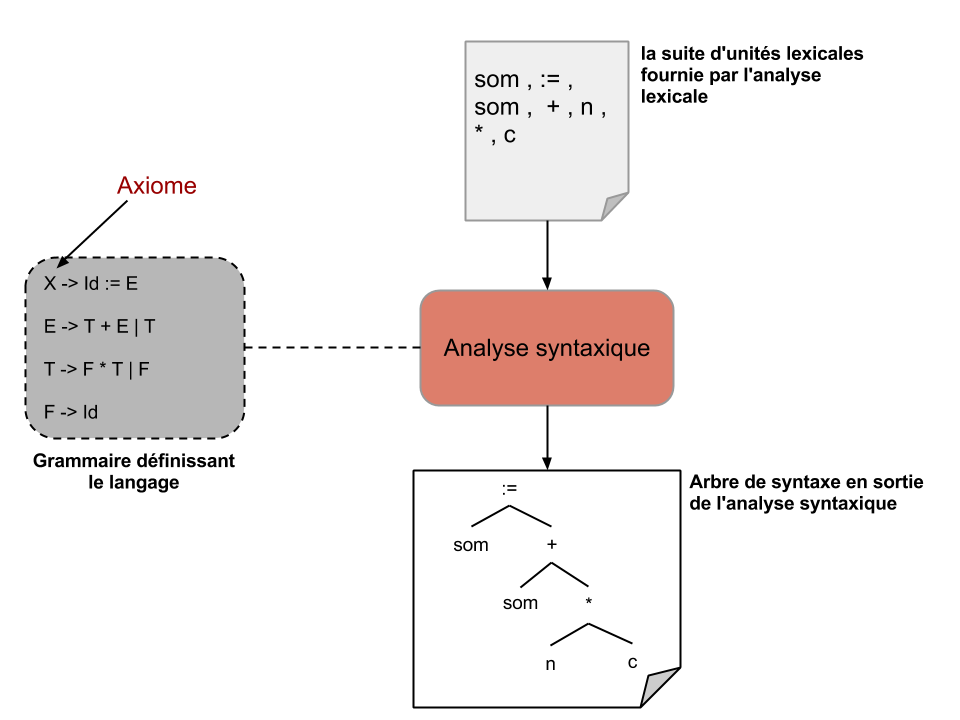
\includegraphics[width=0.65\textwidth]{AnalyseSyntaxique.png}
		\caption{Analyse lexicale}
		\label{fig:AnalyseLexicale}
	\end{figure}\FloatBarrier

\end{frame}

\begin{frame}\frametitle{Analyse Syntaxique}\framesubtitle{Exemple}

	S => S ; S\newline
	S => id := E\newline
	S => print(L)\newline
	E => id\newline
	E => num\newline
	E => E + E\newline
	E => (S , E)\newline
	L => E\newline
	L => L , E\newline\newline

	id := num; id := id + (id := num + num, id)

\end{frame}

\begin{frame}\frametitle{Analyse Syntaxique}\framesubtitle{Exemple}

	\newline\newline
	\underline{S}\newline
	S ; \underline{S}\newline
	\underline{S} ; id := E\newline
	id := \underline{E} ; id := E\newline
	id := num ; id := \underline{E}\newline
	id := num ; id := E + \underline{E}\newline
	id := num ; id := \underline{E} + (S , E )\newline
	id := num ; id := id + (\underline{S} , E )\newline
	id := num ; id := id + (id := \underline{E} , E )\newline
	id := num ; id := id + (id := E + E , \underline{E} )\newline
	id := num ; id := id + (id := \underline{E} + E , id )\newline
	id := num ; id := id + (id := num + \underline{E} , id )\newline
	id := num ; id := id + (id := num + num , id )\newline

\end{frame}

\subsection{Analyse LL}

\begin{frame}\frametitle{Analyse LL}\framesubtitle{Définition}

	\begin{itemize}
				\item Left to right\newline
				\item Rightmost derivation\newline
				\item LL(k)\newline
	\end{itemize}

\end{frame}

\begin{frame}\frametitle{Analyse LL}\framesubtitle{Exemple}

	mot analysé:   id := num ; id := id + (id := num + num, id)

	\newline\newline
	\underline{S}\newline
	\underline{S} ; S\newline
	id := \underline{E} ; S\newline
	id := num ; \underline{S}\newline
	id := num ; id := \underline{E}\newline
	id := num ; id := \underline{E} + E\newline
	id := num ; id := id + \underline{E}\newline
	id := num ; id := id + (\underline{S}, E)\newline
	id := num ; id := id + (id := \underline{E} , E)\newline
	id := num ; id := id + (id := \underline{E} + E, E)\newline
	id := num ; id := id + (id := num + \underline{E}, E)\newline
	id := num ; id := id + (id := num + num, \underline{E})\newline
	id := num ; id := id + (id := num + num, id)\newline

\end{frame}

\subsection{Analyse LR}

\begin{frame}\frametitle{Analyse LR}\framesubtitle{Définition}

	\begin{itemize}
				\item Left to right\newline
				\item Leftmost derivation\newline
				\item LR(k)\newline
	\end{itemize}

\end{frame}

\begin{frame}\frametitle{Analyse LR}\framesubtitle{Exemple}

	mot analysé:   id := num ; id := id + (id := num + num, id)

	\newline\newline
	\underline{S}\newline
	S ; \underline{S}\newline
	S ; id := \underline{E}\newline
	S ; id := E + \underline{E}\newline
	S ; id := E + (S, \underline{E})\newline
	S ; id := E + (\underline{S}, id)\newline
	S ; id := E + (id := \underline{E}, id)\newline
	S ; id := E + (id := E + \underline{E}, id)\newline
	S ; id := E + (id := \underline{E} + num, id)\newline
	S ; id := \underline{E} + (id := num + num, id)\newline
	\underline{S} ; id := id + (id := num + num, id)\newline
	id := \underline{E} ; id := id + (id := num + num, id)\newline
	id := num ; id := id + (id := num + num, id)\newline

\end{frame}

\begin{frame}\frametitle{Analyse LR}\framesubtitle{Types d'analyseurs LR}

	\begin{itemize}
				\item Analyseurs LR simples (SLR)\newline
				\item Analyseurs syntaxiques LR avec anticipation (LALR)\newline
				\item Analyseurs syntaxiques canoniques\newline
	\end{itemize}

\end{frame}





% Section 2---------------------------------------------------
\section{Comparaison entre les outils}

\subsection{YACC}

\begin{frame}\frametitle{YACC}\framesubtitle{Définitions}

	\begin{itemize}
				\item Génération d'analyseur syntaxique\newline
						\subitem \textit{A partir d'une spécification}\newline
				\item Langage : C\newline
						\subitem \textit{Les analyseurs syntaxique généré par YACC sont en langage C}\newline
				\item Type LALR\newline
						\subitem \textit{Les analyseurs syntaxique généré par YACC sont de type LALR}\newline
	\end{itemize}

\end{frame}

\begin{frame}\frametitle{YACC}\framesubtitle{Spécifications}

	Les spécifications permettent:

	\begin{itemize}
				\item Description du langage\newline
				\item Spécification des actions associées au règles de grammaires\newline
				\item Génération d'analyseur syntaxique\newline
	\end{itemize}

\end{frame}

\begin{frame}\frametitle{YACC}\framesubtitle{Structure de la spécifications}

La spécification suit la structure suivante :

Bloc des déclarations

%%

Règles de grammaire

%%

Programme

A : B \{ /* action pour cette regle */ \};

\end{frame}

\begin{frame}\frametitle{YACC}\framesubtitle{Exemple}

	\begin{itemize}
		\item Exemple de spécification YACC
				\subitem \textit{Génération d'une calculatrice}\newline
		\item But: Intérprétateur de commande permettant de faire des opération telles que:\newline
				\subitem \textit{2+5}\newline
				\subitem \textit{(1+2)}\newline
				\subitem \textit{1*2}\newline
				\subitem \textit{2*(2+1)}\newline
		\item Plus de simplicité:\newline
				\subitem \textit{les nombres à plusieurs chiffres ne sont pas pris en charge}
	\end{itemize}

\end{frame}

\begin{frame}[fragile,allowframebreaks=0.98]\frametitle{YACC}\framesubtitle{Exemple}

G(L) = <N,X,P,S> Avec
\begin{Verbatim}[fontsize=\scriptsize,frame=lines]
N : { ligne, commande, expr, terme, facteur }
X : { [0-9], \n, +, *, (, ) }
P : {
    ligne -> 		
        commande \n ligne
        | \n
    commande :	
        expr
    expr :		
        expr + terme
        | terme
    terme : 		
        terme * facteur
        | facteur
    facteur : 		
         ( expr )
        | [0-9]
}
S : ligne

\end{Verbatim}

\end{frame}

\begin{frame}[fragile,allowframebreaks=0.98]\frametitle{YACC}\framesubtitle{Exemple}

Fonction yylex():

\begin{Verbatim}[fontsize=\scriptsize,frame=lines]

%{
    #include <ctype.h>
    #include <stdio.h>
    #include <stdlib.h>
%}

%token CHIFFRE

%%
ligne : commande '\n' ligne
    | '\n' { printf("Fin du programme\n"); exit(0); }
    ;

commande: expr { printf("Resultat: %d\n", $1); };


expr : expr '+' terme { $$ = $1 + $3; }
    | terme
    ;
   
terme : terme '*' facteur { $$ = $1 * $3; }
    | facteur
    ;
   
facteur : '(' expr ')' { $$ = $2; }
    | CHIFFRE
    ;

%%
int main(){
    yyparse();   
}

int yyerror(char *s){
    printf("%s \n", s);
}


int yylex(){
    int c;
    c = getchar();
    if(isdigit(c)){
        yylval = c-'0';
        return CHIFFRE;
    }
    return c;
}

\end{Verbatim}

\end{frame}

\begin{frame}\frametitle{YACC}\framesubtitle{Spécifications}

	Pour faire fonctionner cet exemple, il faudra entrer les lignes de commande suivantes:

	\begin{itemize}
				\item > bison exemple1.y\newline
				\item > gcc exemple1.tab.c -o exemple1\newline
				\item > ./exemple1\newline
	\end{itemize}

\end{frame}

\subsection{ANTLR}


\subsubsection{Définition}



\subsubsection{Exemple}


\subsection{Résultat}

\begin{frame}\frametitle{Résultat}

	Yacc(LALR) vs Antlr(LL):
	\begin{itemize}
				\item Récursivité à gauche\newline
				\item complexité d'utilisation\newline
				\item Performance et flexibilité\newline
	\end{itemize}

\end{frame}

% Section 3---------------------------------------------------
\section{Xtext}

\subsection{Définition}



\subsection{Fonctionnement}



\subsection{Exemple}




%-------------------------------------------------------------

\section{Conclusion}

\end{document}

%%% Local Variables: 
%%% mode: latex
%%% TeX-master: t
%%% coding: utf-8
%%% End: 
